\let\negmedspace\undefined
\let\negthickspace\undefined
\documentclass[journal]{IEEEtran}
\usepackage[a5paper, margin=10mm, onecolumn]{geometry}
%\usepackage{lmodern} % Ensure lmodern is loaded for pdflatex
\usepackage{tfrupee} % Include tfrupee package

\setlength{\headheight}{1cm} % Set the height of the header box
\setlength{\headsep}{0mm}     % Set the distance between the header box and the top of the text

\usepackage{gvv-book}
\usepackage{gvv}
\usepackage{cite}
\usepackage{amsmath,amssymb,amsfonts,amsthm}
\usepackage{algorithmic}
\usepackage{graphicx}
\usepackage{textcomp}
\usepackage{xcolor}
\usepackage{txfonts}
\usepackage{listings}
\usepackage{enumitem}
\usepackage{mathtools}
\usepackage{gensymb}
\usepackage{comment}
\usepackage[breaklinks=true]{hyperref}
\usepackage{tkz-euclide} 
\usepackage{listings}
% \usepackage{gvv}                                        
\def\inputGnumericTable{}                                 
\usepackage[latin1]{inputenc}                                
\usepackage{color}                                            
\usepackage{array}                                            
\usepackage{longtable}                                       
\usepackage{calc}                                             
\usepackage{multirow}                                         
\usepackage{hhline}                                           
\usepackage{ifthen}                                           
\usepackage{lscape}
\begin{document}

\bibliographystyle{IEEEtran}
\vspace{3cm}



\title{10.3.6.1.6}
\author{EE24BTECH11020 - Ellanti Rohith}
{\let\newpage\relax\maketitle}

\textbf{QUESTION} : \\
Solve the system of equations$x\neq0,y\neq0$.
\begin{align}
    6x + 3y &= 6xy \label{eq:qn1} \\
    2x + 4y &= 5xy \label{eq:qn2}
\end{align}


\textbf{SOLUTION} : \\
Dividing both equations by $xy$,
\begin{align}
    \frac{6x}{xy} + \frac{3y}{xy} &= \frac{6xy}{xy} \\
    \frac{2x}{xy} + \frac{4y}{xy} &= \frac{5xy}{xy}
\end{align}
which simplifies to
\begin{align}
    \frac{6}{y} + \frac{3}{x} &= 6 \label{eq:trans1} \\
    \frac{2}{y} + \frac{4}{x} &= 5 \label{eq:trans2}
\end{align}
Let $u = \dfrac{1}{x}$ $(x \neq 0)$ and $v = \dfrac{1}{y}(y\neq 0)$. Then the system transforms to
\begin{align}
    6v + 3u &= 6 \label{eq:lin1} \\
    2v + 4u &= 5 \label{eq:lin2}
\end{align}

The matrix form is
\begin{align}
    \myvec{6 & 3 \\ 2 & 4} \myvec{v \\ u} &= \myvec{6 \\ 5}
\end{align}
\[
\myvec{
6 & 3 & 6 \\
2 & 4 & 5
}
\xrightarrow{R_1 \div 6, \ R_2 - 2R_1}
\myvec{1 & \frac{1}{2} & 1 \\
0 & 3 & 3
}\xrightarrow{R_2 \div 3, \ R_1 - \frac{1}{2} R_2}
\myvec{1 & 0 & \frac{1}{2} \\
0 & 1 & 1
}\]

Thus, \( x = \frac{1}{2}, y = 1 \).



\textbf{LU decomposition} : \\
The matrix $\vec{A}$ can be decomposed as
\begin{align}
	\vec{A} &= \vec{L} \vec{U}
\end{align}
where, 
\begin{align}
	\vec{L} &= Lower triangular \\
	\vec{U} &= Upper triangular
\end{align}
Then the system of equations can be solved as
\begin{align}
	\vec{A} \vec{x} &= \vec{B} \label{eq:solve}\\
	\vec{L} \vec{U} \vec{x} &= \vec{B} \\
	\implies \vec{L} \vec{y} &= \vec{B} \label{eq:lu1} \\
	\vec{U} \vec{x} &= \vec{y} \label{eq:lu2}
\end{align}
\textbf{Algorithm} : \\
\begin{enumerate}
	\item Let $\vec{A}$ be an $n \times n$ matrix. Initialize $\vec{L}$ to an $n \times n$ Identity matrix. Initialize $\vec{U}$ to a zero matrix.
	\begin{align}
		L &= \myvec{1 & 0 & \cdots & 0 \\
		            0 & 1 & \cdots & 0 \\
		            \vdots & \vdots & \ddots & \vdots \\
		            0 & 0 & \cdots & 1} \\
		U &= \myvec{0 & 0 & \cdots & 0 \\
			    0 & 0 & \cdots & 0 \\
                            \vdots & \vdots & \ddots & \vdots \\
                            0 & 0 & \cdots & 0}
	\end{align}
	\item For each row $i$ from $0$ to $n-1$ :
	\begin{enumerate}
		\item For each column $j$ from $i$ to $n-1$ : 
		\begin{align}
			U_{ij} &= A_{ij} - \sum_{k=0}^{i-1} L_{ik} U_{kj}
		\end{align}
		\item For each row $j$ from $i+1$ to $n-1$ :
		\begin{align}
			L_{ji} &= \frac{1}{U_{ii}} \brak{A_{ij} - \sum_{k=0}^{i-1} L_{jk} U_{ki}}
		\end{align}
	\end{enumerate}
	\item Repeat the above step for all $i = 0,1,\dots,n-1$
	\item After all the iterations
	\begin{align}
		\vec{A} &= \vec{L} \vec{U}
	\end{align}
\end{enumerate}
Decomposing $\vec{A}$ as $\vec{L}\vec{U}$,
\begin{align}
    \vec{L} &= \myvec{1 & 0 \\ \frac{1}{3} & 1}, \quad \vec{U} = \myvec{6 & 3 \\ 0 & 3}
\end{align}
Using forward substitution,
\begin{align}
    \myvec{1 & 0 \\ \frac{1}{3} & 1} \myvec{y_1 \\ y_2} &= \myvec{6 \\ 5}
\end{align}
Solving,
\begin{align}
    y_1 &= 6, \quad y_2 = 5 - \frac{1}{3} \times 6 = 3
\end{align}
Using backward substitution,
\begin{align}
    \myvec{6 & 3 \\ 0 & 3} \myvec{v \\ u} &= \myvec{6 \\ 3}
\end{align}
Solving,
\begin{align}
    u &= 1, \quad v = \frac{6 - 3(1)}{6} = \frac{1}{2}
\end{align}
Thus,
\begin{align}
    \frac{1}{x} = 1 \implies x = 1, \quad \frac{1}{y} = \frac{1}{2} \implies y = 2
\end{align}

\textbf{QR decomposition} : \\
Decomposing $\vec{A}$ as $\vec{Q}\vec{R}$,
\begin{align}
    \vec{Q} &= \myvec{\frac{6}{\sqrt{45}} & \frac{3}{\sqrt{45}} \\ \frac{2}{\sqrt{5}} & \frac{4}{\sqrt{5}}}, \\
    \vec{R} &= \myvec{\sqrt{45} & \sqrt{5} \\ 0 & \frac{6}{\sqrt{5}}}
\end{align}
The system simplifies as:
\begin{align}
    \vec{R} \myvec{v \\ u} &= \vec{Q}^{T} \myvec{6 \\ 5}
\end{align}
Computing,
\begin{align}
    \myvec{\sqrt{45} & \sqrt{5} \\ 0 & \frac{6}{\sqrt{5}}} \myvec{v \\ u} &= \myvec{\frac{6}{\sqrt{45}} & \frac{3}{\sqrt{45}} \\ \frac{2}{\sqrt{5}} & \frac{4}{\sqrt{5}}}^{T} \myvec{6 \\ 5}
\end{align}
Solving for $u, v$:
\begin{align}
    u &= 1, \\
    v &= \frac{1}{2}
\end{align}

Hence, the system is \textbf{consistent} with a unique solution $x=1$, $y=2$. 
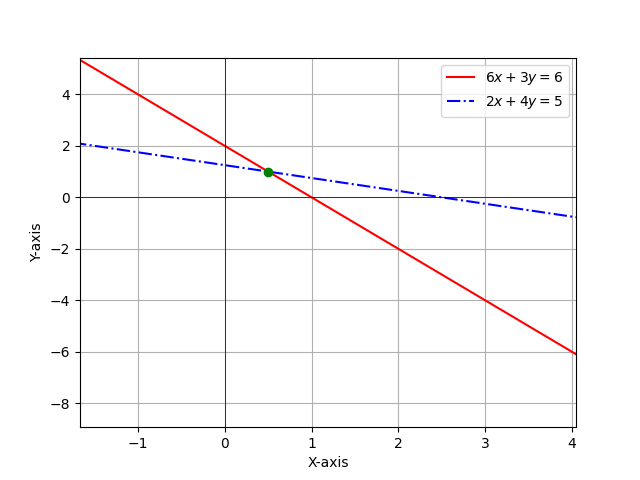
\includegraphics[width=\textwidth]{Figs/Figure_1.png}
\end{document}
